\documentclass[class=report,crop=false, 12pt]{standalone}
\usepackage[screen,nosolutions]{../scratch}

%\usepackage[print]{../scratch}

\begin{document}

\titre[S]{Coordonnées $x,y$}
%===============================

\insertvideo{bZGv9CRfkuI}{Coordonnées $x,y$ -- Activité 1}

\insertvideo{3_MUTUTAHJg}{Coordonnées $x,y$ -- Activité 2}

\insertvideo{-FGNNU4qdMw}{Coordonnées $x,y$ -- Activité 3}

\bigskip
\bigskip


\begin{activite}

Essaie de reproduire la spirale suivante.

\begin{center}
  \includegraphics[scale=\scaleecran,scale=1.1]{ecran-03-ex1}   
\end{center}

Au départ la taille du stylo est 1.
Fais une boucle dans laquelle à chaque étape :
\begin{itemize}
  \item Scratch avance de 6 pas,
  \item puis tourne de 3 degrés vers la gauche,
  \item puis ajoute 1 à la taille du stylo,
  \item puis ajoute 1 à la couleur du stylo.
\end{itemize}


Trouve une bonne position $x,y$ de départ afin que la spirale tienne entièrement dans l'écran.



%\textbf{Blocs utiles.}
%\begin{itemize}
%  \item 
%  
%  \item 
%  
%  
%\end{itemize}

\end{activite}


\begin{activite}
Tu vas programmer ton premier logiciel de dessin.

\begin{center}
  \includegraphics[scale=\scaleecran,scale=0.9]{ecran-03-ex2}   
\end{center}

Pour cela, construis une boucle qui répète indéfiniment :
\begin{itemize}
  \item aller au pointeur de la souris,
  \item afficher l'abscisse $x$ pendant 1 seconde,
  \item afficher l'ordonnée $y$ pendant 1 seconde.
\end{itemize}

Essaie de dessiner un escargot, une maison, une fusée...

\bigskip

\textbf{Blocs utiles.}
\begin{itemize}
  \item Aller à \og pointeur de la souris \fg{}
  \item Dire \og abscisse $x$ \fg{} pendant 1 seconde
\end{itemize}

\bigskip

\textbf{Bonus.}
\begin{itemize}
  \item Change de couleur à chaque segment.
  \item Affiche $x$ et $y$ en même temps.
\end{itemize}
\end{activite}


\begin{activite}

Choisis comme arrière-plan la grille de coordonnées.

\begin{enumerate}
  \item Trace le chiffre \og \mot{4} \fg{} en suivant les instructions suivantes :
  \begin{itemize}
    \item relever le stylo,
    \item aller à $x=40$, $y=120$,
    \item stylo en position d'écriture,
    \item aller à $x=0$, $y=40$,
    \item aller à $x=80$, $y=40$,
    \item relever le stylo,
    \item aller à $x=60$, $y=20$,
    \item stylo en position d'écriture,
    \item aller à $x=60$, $y=60$.  
  \end{itemize}
  
\begin{center}
  \includegraphics[scale=\scaleecran,scale=0.7]{ecran-03-ex3}   
\end{center}
  
  \item Trace le chiffre \og \mot{7} \fg{} en t'aidant des coordonnées $(x,y)$ des sommets proposés dans le dessin suivant : 
  
\myfigure{0.5}{
\footnotesize\tikzinput{coord1}
}  

  \item Dessine la première lettre de ton prénom en majuscule sur la grille ci-dessous.

\myfigure{1}{
\small\tikzinput{coord2}
}  
  
  \item Programme Scratch afin qu'il dessine ton initiale.
  
  
\end{enumerate}


\end{activite}


\ifx \displaysolutions \myzero
\else
\begin{code}
\onesolution{Coordonnées $x,y$}{Activité 1}{\includegraphics[scale=\scalesolution]{code-03-ex1}}
\onesolution{Coordonnées $x,y$}{Activité 2}{\includegraphics[scale=\scalesolution]{code-03-ex2}}
\onesolution{Coordonnées $x,y$}{Activité 3}{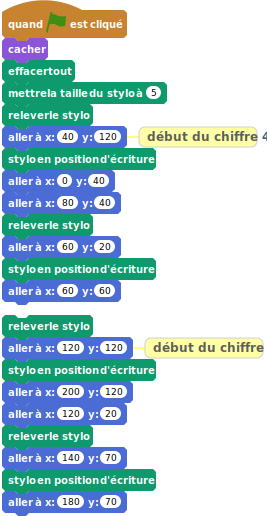
\includegraphics[scale=\scalesolution]{code-03-ex3}}    
\end{code}
\fi

\end{document}

